\documentclass[a4paper]{article}
\usepackage{amsfonts}
\usepackage{amsmath}
\usepackage{amssymb}
\usepackage{graphicx}     

\begin{document}
  
\noindent \large Auteur: Victoria Mazur \\
\noindent \large Studierichting: Informatica\\
\noindent \large Oefeningenreeks 5D nr. 3.3\\

\medskip

\normalsize

$f(x) - g(x) = x^2 + 4x - x + 2$ \\

$= x^2 + 3x + 2$ \\

Snijpunten zoeken: $x^2 + 3x + 2 = 0$ \\

Som en product van wortels: \\

Som: $x_1 + x_2 = -\dfrac{b}{a} = -\dfrac{3}{1} = -3$ \\

Product: $x_1 \cdot x_2 = \dfrac{c}{a} = \dfrac{2}{1} = 2$ \\

Zoeken naar twee getallen met som $-3$ en product $2$: \\

$\Rightarrow x_1 = -1, x_2 = -2$ \\

Oppervlakte bepalen per interval: \\

$\displaystyle\int_{-3}^{-2} (x^2 + 3x + 2)dx + \displaystyle\int_{-2}^{-1} (x^2 + 3x + 2)dx + \displaystyle\int_{-1}^{0} (x^2 + 3x + 2)dx$ \\

Primitieve: $\displaystyle\int (x^2 + 3x + 2)dx = \dfrac{x^3}{3} + \dfrac{3x^2}{2} + 2x$ \\

$= \left[ \dfrac{x^3}{3} + \dfrac{3x^2}{2} + 2x \right]_{-3}^{-2} - \left[ \dfrac{x^3}{3} + \dfrac{3x^2}{2} + 2x \right]_{-2}^{-1} + \left[ \dfrac{x^3}{3} + \dfrac{3x^2}{2} + 2x \right]_{-1}^{0}$ \\

Evalueren van grenzen: \\

Bij $x = -2$: $\dfrac{(-2)^3}{3} + \dfrac{3(-2)^2}{2} + 2(-2) = -\dfrac{8}{3} + 6 - 4 = -\dfrac{8}{3} + 2 = \dfrac{-8+6}{3} = -\dfrac{2}{3}$ \\

Bij $x = -3$: $\dfrac{(-3)^3}{3} + \dfrac{3(-3)^2}{2} + 2(-3) = -9 + \dfrac{27}{2} - 6 = -15 + \dfrac{27}{2} = \dfrac{-30+27}{2} = -\dfrac{3}{2}$ \\

$= -\left(-\dfrac{2}{3} + \dfrac{3}{2}\right) - \left(-\dfrac{5}{6} + \dfrac{3}{3}\right) - \left(-\dfrac{5}{6}\right)$ \\

$= \dfrac{11}{6}$ \\

\begin{figure}[h]
\centering
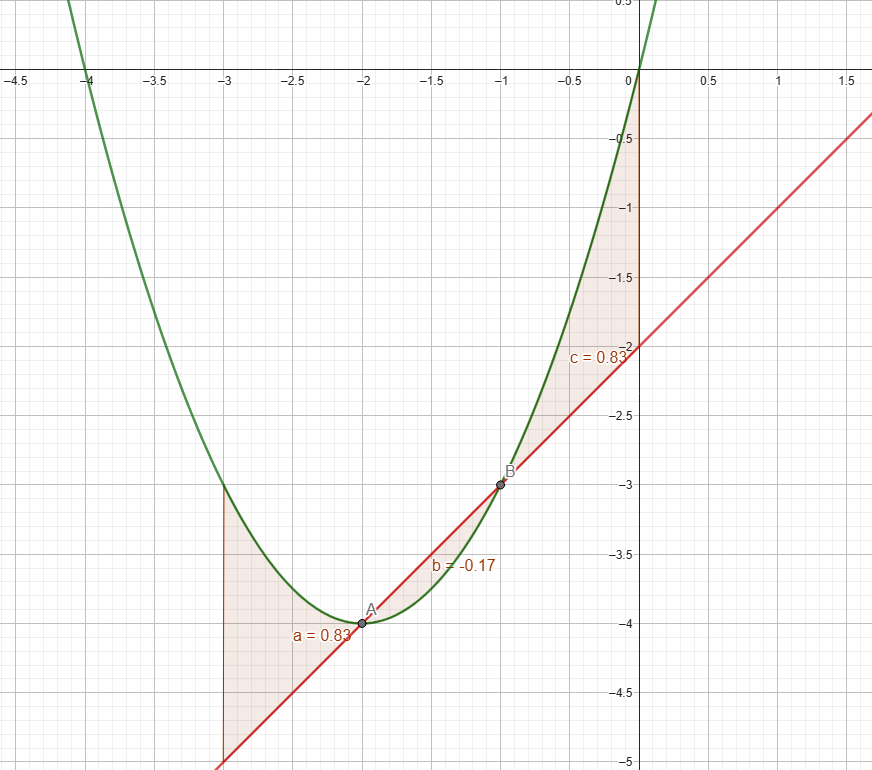
\includegraphics[width=10cm]{5D-3.3-victoria.mazur.INF.png}
\end{figure}

\begin{thebibliography}{999}
%\bibitem{a} Referentie
\end{thebibliography}
\end{document}